\documentclass[unknownkeysallowed,xcolor=table]{beamer}
 
\usepackage [T2A,T1] {fontenc}
\usepackage[utf8]{inputenc}
\usepackage[english,russian]{babel}
\usepackage{amsmath}
\usepackage{pifont}
\usepackage{listings}
\usepackage{url}
\usepackage{textcomp}

\setbeamertemplate{navigation symbols}{}

\newcommand{\textapprox}{\raisebox{0.5ex}{\texttildelow}}

\colorlet{mygreen}{green!60!blue}
\colorlet{mymauve}{red!60!blue}

\lstset{
      basicstyle=\ttfamily\small,
      commentstyle=\color{mygreen},
      keywordstyle=\color{blue},
      numberstyle=\tiny\color{blue},
      stringstyle=\color{mymauve},
      numbers=left,
      stepnumber=1,
      columns=fullflexible,
      breaklines=true,
      postbreak=\mbox{\textcolor{red}{\ensuremath{\hookrightarrow}\space}},
      literate={~} {\textapprox}{1},
      language={[11]C++}
}

\makeatletter
\newcommand{\srcmediumsize}{\@setfontsize{\srcmediumsize}{7pt}{7pt}}
\makeatother

\makeatletter
\newcommand{\srcbigsize}{\@setfontsize{\srcbigsize}{8pt}{8pt}}
\makeatother

\makeatletter
\newcommand{\srcsize}{\@setfontsize{\srcsize}{6pt}{6pt}}
\makeatother

\makeatletter
\newcommand{\srcsmallsize}{\@setfontsize{\srcsmallsize}{5pt}{5pt}}
\makeatother

\title[C++]
{Программирование на языке C++}
 
\subtitle{Unit testing}
 
\author[А.~Б.~Морозов]
{
  \texorpdfstring{Александр Морозов\newline\href{mailto:gelu.speculum@gmail.com}{gelu.speculum@gmail.com}}
  {Александр Морозов}
}

\date[ITMO 2020]
{ИТМО, осенний семестр 2020}
  
\logo{%
  \makebox[0.97\paperwidth]{%
    
\includegraphics[align=c,width=2cm,keepaspectratio]{itmo_logo.png}
    \hfill
    
\includegraphics[align=c,width=1.5cm,keepaspectratio]{itiviti_logo.png}
  }
}

\AtBeginSection[]
{
  \begin{frame}
    \frametitle{Содержание}
    \tableofcontents[currentsection]
  \end{frame}
}

\begin{document}

\section{Общие вопросы тестирования}

\begin{frame}{Виды тестирования}
  \begin{itemize}
    \item ручное \vspace{0.5em}
    \item автоматическое
  \end{itemize}
  \vspace{2em}
  \begin{itemize}
    \item функциональное тестирование продукта целиком \vspace{0.5em}
    \item функциональное тестирование компонент продукта \vspace{0.5em}
    \item нагрузочное тестирование \vspace{0.5em}
    \item стресс тестирование \vspace{0.5em}
    \item юнит тестирование
  \end{itemize}
\end{frame}

\begin{frame}{Монолит}
  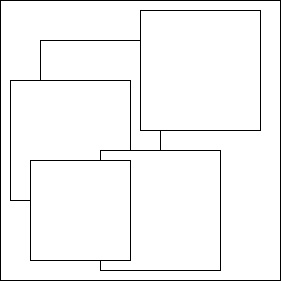
\includegraphics[align=c,width=7cm,keepaspectratio]{images/unit_testing/monolith.png}
\end{frame}

\begin{frame}{Полносвязная система}
  
\includegraphics[align=c,width=7cm,keepaspectratio]{images/unit_testing/interconnected.png}
\end{frame}

\begin{frame}{Полносвязная система}
  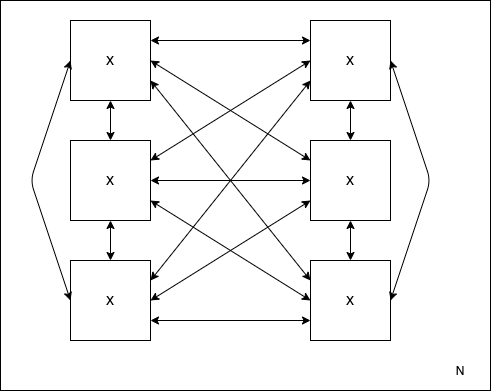
\includegraphics[align=c,width=7cm,keepaspectratio]{images/unit_testing/interconnected_caption.png}
\end{frame}

\begin{frame}{Неопределённо связная система}
  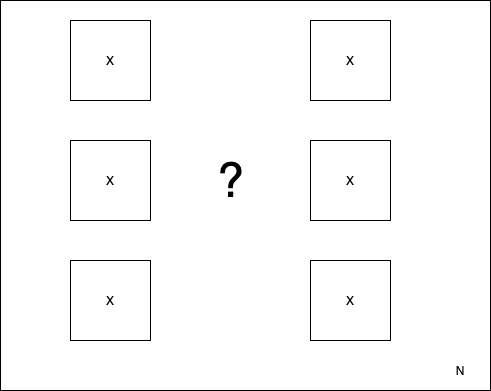
\includegraphics[align=c,width=7cm,keepaspectratio]{images/unit_testing/unknown.png}
\end{frame}

\begin{frame}{Комбинаторная сложность}
  \begin{itemize}
    \item невозможно (невыполнимо) проверить все возможные состояния \vspace{2em}
    \item сложно предсказать ``значимые'' и ``малозначимые'' состояния \vspace{2em}
    \item стохастическое тестирование \url{https://hackage.haskell.org/package/QuickCheck}
  \end{itemize}
\end{frame}

\begin{frame}{Степень покрытия}
  \begin{itemize}
    \item процент строк исходного кода, выполненные в ходе прогона тестов \vspace{2em}
    \item gcov, llvm-gcov
  \end{itemize}
\end{frame}

\section{GTest}

\begin{frame}{GTest}
  \url{https://github.com/google/googletest}

  \vspace{2em}
  \begin{itemize}
    \item наборы тестов
    \item проверка ожиданий
    \item fixtures
    \item параметризованные тесты
  \end{itemize}
\end{frame}

\section{GMock}

\begin{frame}[fragile]{Хотим протестировать}
  \begin{lstlisting}
  class MdHandler
  {
  public:
    MdHandler(IService & service);
    void handle_packet(const Packet & packet);
    void handle_resend(const Packet & packet);

  private:
    IService & m_service;
  };
  \end{lstlisting}
\end{frame}

\begin{frame}[fragile]{Не хватает реализации}
  \begin{lstlisting}
  class IService
  {
  public:
    virtual ~IService() = default;

    virtual void resend_messages(uint32_t start_seq_num, uint16_t msg_count) = 0;
    virtual void handle_message(uint32_t seq_num) = 0;
  };
  \end{lstlisting}
\end{frame}

\begin{frame}[fragile]{Решение - мок}
  \begin{lstlisting}
  #include <gmock/gmock.h>

  class MockService : public IService
  {
  public:
    MOCK_METHOD(void, resend_messages, (uint32_t, uint16_t));
    MOCK_METHOD(void, handle_message, (uint32_t));
  };
  \end{lstlisting}
\end{frame}

\begin{frame}[fragile]{Использование в тестах}
  \begin{lstlisting}[basicstyle=\ttfamily\srcsize]
  #include <gmock/gmock.h>
  #include <gtest/gtest.h>

  class MdHandlerTest : public ::testing::Test
  {
  public:
    MdHandlerTest()
      : m_handler(m_mock_service)
    { }

    void expect_messages(const uint32_t start_seq_num, const uint32_t end_seq_num)
    {
      uint32_t seq_num = start_seq_num;
      while (seq_num <= end_seq_num) {
        EXPECT_CALL(m_mock_service, handle_message(seq_num++))
          .Times(Exactly(1));
      }
    }
  private:
    MockService m_mock_service;
    MdHandler m_handler;
  };

  TEST_F(MdHandlerTest, no_gaps)
  {
    expect_messages(1, 3);
    ...
  }
  \end{lstlisting}
\end{frame}

\begin{frame}[fragile]{Указание спецификаторов}
  \begin{lstlisting}
  class Real
  {
  public:
    virtual int compute() const = 0;
  };

  class Mock : public Real
  {
  public:
    MOCK_METHOD(int, compute, (), (const, override));
  };
  \end{lstlisting}
\end{frame}

\begin{frame}[fragile]{Некоторые сложности}
  \begin{lstlisting}
  class Mock : public Real
  {
  public:
    MOCK_METHOD(std::pair<int, bool>, foo, ());
  };
  \end{lstlisting}
\end{frame}

\begin{frame}[fragile]{Моки новых методов}
  \begin{lstlisting}
  class MockService : public IService
  {
  public:
    MOCK_METHOD(void, handle_message, (uint32_t), (override));

    MOCK_METHOD(void, on_destroy, ()); // not in IService

    ~MockService() { on_destroy(); }
  };
  \end{lstlisting}
\end{frame}

\begin{frame}[fragile]{Поведение по умолчанию}
  \begin{lstlisting}
  TEST(Foo, bar)
  {
    Mock m;
    ON_CALL(m, process(_))
        .WillByDefault(Return(11));
  }
  \end{lstlisting}
\end{frame}

\begin{frame}[fragile]{Ожидания}
  \begin{lstlisting}
  TEST(Foo, bar)
  {
    Mock m;
    EXPECT_CALL(m, process(_))
        .WillOnce(Return(11))
        .WillRepeatedly(Return(0));
    EXPECT_CALL(m, process(5))
        .WillOnce(Return(-5));
  }
  \end{lstlisting}
\end{frame}

\begin{frame}[fragile]{Matchers}
  \begin{lstlisting}
  TEST_F(FooTest, bar)
  {
    EXPECT_CALL(foo, process(_, Gt(10)));
    EXPECT_CALL(foo,
        send(
            AllOf(
                StartsWith("Abc"),
                Not(HasSubstr("123")))));
  }
  \end{lstlisting}
\end{frame}

\begin{frame}[fragile]{Actions}
  \begin{lstlisting}
  \end{lstlisting}
\end{frame}

\section{Некоторые проблемы юнит-тестов и моков}

\begin{frame}[fragile]{Плохо тестируемый класс}
  \begin{lstlisting}
  class Handler : public HandlerBase
  {
  public:
    Handler(Component &, Service &);

  private:
    Component & m_component;
    Service & m_service;
  };
  \end{lstlisting}
\end{frame}

\begin{frame}[fragile]{Вариант решения - абстрактные интерфейсы}
  \begin{lstlisting}
  class Handler : public HandlerBase
  {
  public:
    Handler(IComponent &, IService &);

  private:
    IComponent & m_component;
    IService & m_service;
  };
  \end{lstlisting}
\end{frame}

\begin{frame}[fragile]{Вариант решения - шаблонизация}
  \begin{lstlisting}
  template <class ComponentT, class ServiceT>
  class HandlerImpl : public HandlerBase
  {
  public:
    HandlerImpl(ComponentT &, ServiceT &);

  private:
    ComponentT & m_component;
    ServiceT & m_service;
  };

  using Handler = HandlerImpl<Component, Service>;
  \end{lstlisting}
\end{frame}

\begin{frame}[fragile]{Вариант решения - шаблонная реализация}
  \begin{lstlisting}[basicstyle=\ttfamily\srcbigsize]
  template <class ComponentT, class ServiceT>
  class HandlerImpl
  {
  public:
    void handle();
  };

  class Handler : public HandlerBase
  {
  public:
    Handler(Component & c, Service & s)
      : m_impl(c, s)
    { }

    void handle()
    {
      m_impl.handle();
    }
  private:
    HandlerImpl<Component, Service> m_impl;
  };
  \end{lstlisting}
\end{frame}

\end{document}
